\documentclass[10pt]{article}
\usepackage[usenames]{color} %used for font color
\usepackage{amssymb} %maths
\usepackage{amsmath} %maths
\usepackage[utf8]{inputenc} %useful to type directly diacritic characters
\usepackage{tikz}
\usepackage{lscape}
\usetikzlibrary{shapes,arrows,snakes,backgrounds,chains}
\tikzstyle{AG} = [rectangle, draw, fill=black!21, 
    text width=6em, text centered, minimum height=4em]
\tikzstyle{AGwide} = [rectangle, draw, fill=black!21, 
    text width=8em, text centered, minimum height=4em]
\tikzstyle{PO} = [rectangle, draw, fill=black!10, 
    text width=6em, text centered, rounded corners, minimum height=4em]
\tikzstyle{POwide} = [rectangle, draw, fill=black!10, 
    text width=8em, text centered, rounded corners, minimum height=4em]
\tikzstyle{line} = [draw, -latex']
\tikzstyle{cloud} = [draw, ellipse,fill=black!1, node distance=3cm, text width=3.5em, text centered,
    minimum height=2em]\begin{document}
\begin{align*}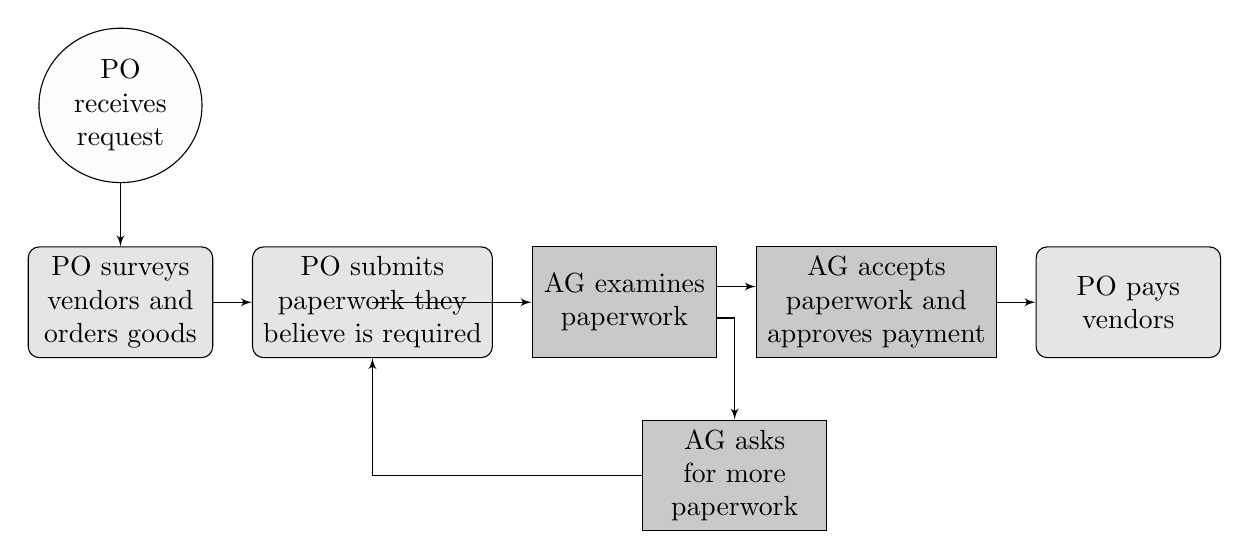
\begin{tikzpicture}[node distance = 2cm, auto]
 \node [PO] (survey) {PO surveys vendors and orders goods};
    \node [cloud, above of=survey, node distance=2.5cm] (request) {PO receives request};
    \node [POwide, right of=survey, node distance=3.2cm] (paperwork) {PO submits paperwork they believe is required};
    \node [AG, right of=paperwork, node distance=3.2cm] (examine) {AG examines paperwork};
    \node at (7.8, -2.2) [AG, name=reject] {AG asks for more paperwork};
    \node [AGwide, right of=examine, node distance=3.2cm] (approve) {AG accepts paperwork and approves payment};
    \node [PO, right of=approve, node distance=3.2cm] (pay) {PO pays vendors};
 \path [line] (survey) -- (paperwork);
    \path [line] (paperwork) |- (examine);
    \path [line] ([yshift=.2cm]examine.east) -- ([yshift=.2cm]approve.west);
    \path [line] ([yshift=-.2cm]examine.east) -| (reject.north);
    \path [line] (reject) - | (paperwork);
    \path [line] (request) -- (survey);
    \path [line] (approve) -- (pay);
\end{tikzpicture}\end{align*}
\end{document}